\documentclass[10pt,twocolumn,letterpaper]{article}

\usepackage{cvpr}
\usepackage{times}
\usepackage{epsfig}
\usepackage{graphicx}
\usepackage{amsmath}
\usepackage{amssymb}

% Include other packages here, before hyperref.

% If you comment hyperref and then uncomment it, you should delete
% egpaper.aux before re-running latex.  (Or just hit 'q' on the first latex
% run, let it finish, and you should be clear).
\usepackage[breaklinks=true,bookmarks=false]{hyperref}

\cvprfinalcopy % *** Uncomment this line for the final submission

\def\cvprPaperID{****} % *** Enter the CVPR Paper ID here
\def\httilde{\mbox{\tt\raisebox{-.5ex}{\symbol{126}}}}

% Pages are numbered in submission mode, and unnumbered in camera-ready
%\ifcvprfinal\pagestyle{empty}\fi
\setcounter{page}{1}
\begin{document}

%%%%%%%%% TITLE
\title{Multiple Cars Detection and Tracking Basing on Kalman Filter}

\author{Kaiyu Zhang\\
A53247294\\
{\tt\small kaz082@eng.ucsd.edu}
% For a paper whose authors are all at the same institution,
% omit the following lines up until the closing ``}''.
% Additional authors and addresses can be added with ``\and'',
% just like the second author.
% To save space, use either the email address or home page, not both
\and
Shihao Luo\\
A53254332\\
{\tt\small shl667@eng.ucsd.edu}
\and
Pengluo Wang\\
A53247710\\
{\tt\small pew067@eng.ucsd.edu}
}
\maketitle
%\thispagestyle{empty}

%%%%%%%%% ABSTRACT
\begin{abstract}
We present an algorithm and its implementation of detection and tracking of multiple vehicles using a mounted camera inside a self-driving car applying Kalman filter. It was developed as an application of Kalman filter and is intended to provide convenience for automatic car driving in real world. Tracking is done by combining prediction and correction process with a
Kalman filter. No ground plane
assumption is made. The resulting system runs at frame rate or higher, and produces excellent estimates of multiple tracked vehicle. We used TensorFlow Object Detection API, which is an open source framework built on top of TensorFlow to construct, train and deploy object detection models. previous CVPR abstracts to get a feel for style and length.
\end{abstract}

%%%%%%%%% BODY TEXT
\section{Introduction}

Within the last few years, research into intelligent vehicles has expanded into applications that work with or for the human user. Human-factors research is merging with intelligent-vehicle technology to create a new generation of driver-assistance systems that go beyond automated control systems by attempting to work in harmony with a human operator. Tracking objects in image sequences is an important task for
vehicle guidance, following moving objects or to obtain a description
of an environment. We need promote the accuracy of car tracking to provide convenience for car driving. In most systems the first step in
tracking objects is to separate the foreground from the background
or to detect motion. This means to detect the regions
(apparent shape) of independently moving objects regardless
of their speed, direction or texture. In this work we illustrate the detection and tracking of multiple vehicles using a mounted camera inside a self-driving car. 

The data we use is a set of video taken by the dashcam in front of our car, which is real and reliable. The data was taken in our daily life, including different situations: no cars, one car, more than one cars in the visual area. The cars in the video have several typical behaviours including intersection and overtaking.

This paper first initializes a detector for sensing target maneuvers and then develops the combination of the estimator, detector, and a Kalman filter to form a tracker for maneuvering targets. The detector localizes the vehicles in each video frame, the tracker is then updated with the detection results. Finally the tracking results are annotated and displayed in a video frame.

Section 2 gives a brief introduction to the Kalman filter theory
and how to apply it to the background estimation problem.
Extensions of the background estimator used so far are given
in Section 3. Results are presented in Section 4. Concluding
remarks are given in Section 5.

%------------------------------------------------------------------------
\section{Algorithm and technique}

To implement the tracking algorithm, we separate the problem into two parts: \textbf{detection} and \textbf{prediction}, shown as two bounding box of the car.Then combine them together as the tracking result by adding confidence level to show how much we trust the prediction. In this way we have implemented the whole Tracking algorithm. Next, we will introduce the main idea and theory of the two algorithms

%-------------------------------------------------------------------------
\subsection{Object detection}

SSD(Single Shot Detection) algorithm is an object detection algorithm that directly predicts the coordinates and categories of the objection with bounding box, which is much faster than those traditional detection models without losing the accuracy, by adding several separate prediction filters. In this project, we use the open source with a trained model to process each frames of the video data to implement the detection.

%-------------------------------------------------------------------------
\subsubsection{Tensor flow object detection API}

Creating accurate deep learning models capable of localizing and identifying multiple objects in a single image remains a core challenge in computer vision. TensorFlow Object Detection API is an open source framework built on top of TensorFlow that makes it easy to construct, train and deploy object detection models. This API is developed by Google research team, including: boosted trees, mnist, resnet, wide deep, single shot detection and etc. models. Each model has already been trained on different dataset.

%-------------------------------------------------------------------------
\subsubsection{Single shot detection(SSD) briefly introduction}

SSD~\cite{SSD} is a method for detecting objects in images using a single
deep neural network. It discretized the output space of
bounding boxes into a set of default boxes over different aspect ratios and scales
per feature map location. At prediction time, the network generates scores for the
presence of each object category in each default box and produces adjustments to
the box to better match the object shape. Additionally, the network combines predictions
from multiple feature maps with different resolutions to naturally handle
objects of various sizes. SSD is simple relative to methods that require object
proposals because it completely eliminates proposal generation and subsequent
pixel or feature re-sampling stages and encapsulates all computation in a single
network. This makes SSD easy to train and straightforward to integrate into systems
that require a detection component. 
\begin{figure}[t]
\begin{center}
   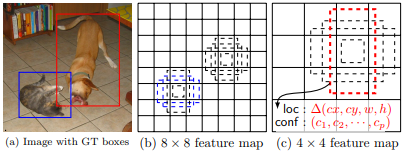
\includegraphics[width=1\linewidth]{model1}
\end{center}
   \caption{Basic idea of SSD}
\label{fig:2_1_1}
\end{figure}

Figure \ref{fig:2_1_1} is the SSD framework. (a) SSD only needs an input image and ground truth boxes for each object during training. In a convolutional fashion, we evaluate a small set (e.g. 4) of default boxes of different aspect ratios at each location in several feature maps with different scales (e.g. $8 \times 8$ and $4 \times 4$ in (b) and (c)). For each default box, we predict both the shape offsets and the confidences for all object categories ((c1, c2, ...,  cp)). At training time, we first match these default boxes to the ground truth boxes. For example, we have matched two default boxes with the cat and one with the dog, which are treated as positives and the rest as negatives. The model loss is a weighted sum between localization loss (e.g. Smooth L1 [6]) and confidence loss (e.g. Softmax).

The SSD approach is based on a feed-forward convolutional network that produces
a fixed-size collection of bounding boxes and scores for the presence of object class
instances in those boxes, followed by a non-maximum suppression step to produce the
final detections. The early network layers are based on a standard architecture used for
high quality image classification (truncated before any classification layers), which we
will call the base network2
. We then add auxiliary structure to the network to produce
detections with the following key features:
\\(1) Multi-scale feature maps for detection;
\\(2) Constitutional predictors for detection.
\\ 
In the TensorFlow Object Detection API, the model has been trained on CoCo dataset, with different labeled objects. The Labeled ID with objection are shows in Table.1. \\

\begin{table}
\begin{center}
\begin{tabular}{|c|c|}
\hline
ObjectionID & Objection \\
\hline\hline
1 & Person \\
\hline
2 & Bicycle \\
\hline
3 & Car\\
\hline
4 & Motorcycle\\
\hline
5 &Bus \\
\hline
6 & Train \\
\hline
7 & Traffic Light \\
\hline
8 & Stop Sign \\
\hline
\end{tabular}
\end{center}
\caption{Objection ID}
\end{table}
%-------------------------------------------------------------------------
\subsubsection{Car detection}
AS mentioned above, the model SSD has been trained and can detect the object. In our project, we only care about the objects related to transportation. The inputs are the frames of the video. After passing the SSD model, we have three key outputs: (1) objection ID; (2) bounding box information; (3) confidence score. Then we need to judge the output whether it is satisfy our requirement. The detecting object is car with ID(3). Because we want tracking the cars with close distance, the bounding box needs to be big enough and has appropriate ratio(4*3). Besides, the confidence score shows how correct the detection is, which need to above 0.3. The flow chart is shown as figure \ref{fig:2_1_2}.\\
\begin{figure}[t]
\begin{center}
   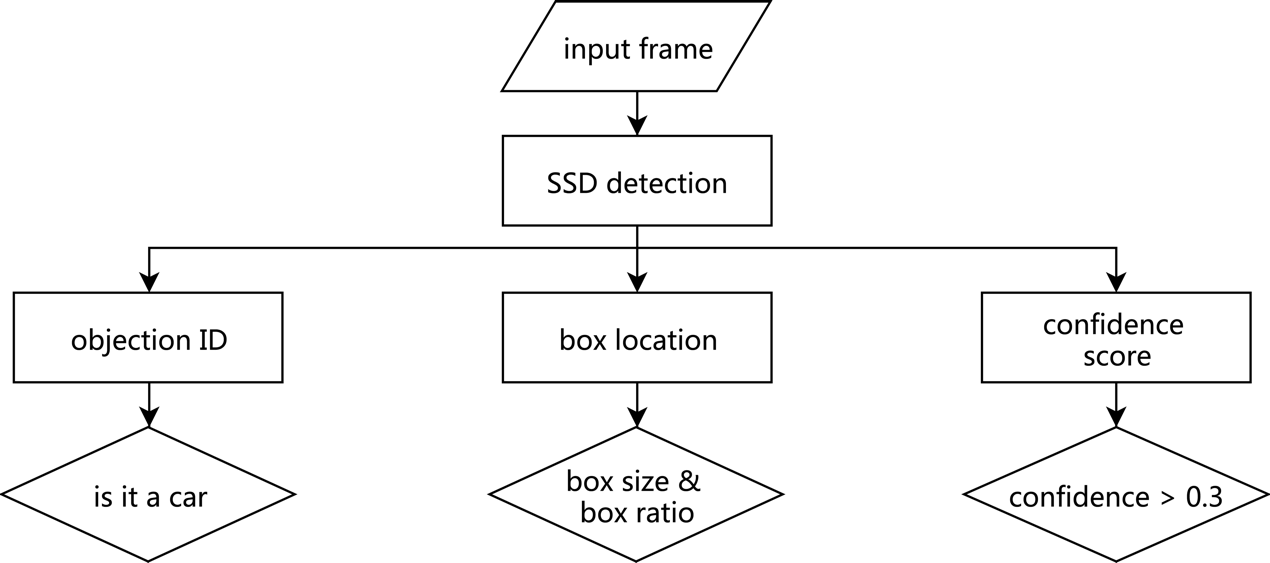
\includegraphics[width=0.9\linewidth]{ssd_chart}
\end{center}
   \caption{Flow chart of SSD}
\label{fig:2_1_2}
\end{figure}
The behavior of SSD detection are shown in figure \ref{fig:2_1_3}.
\begin{figure}[t]
\begin{center}
   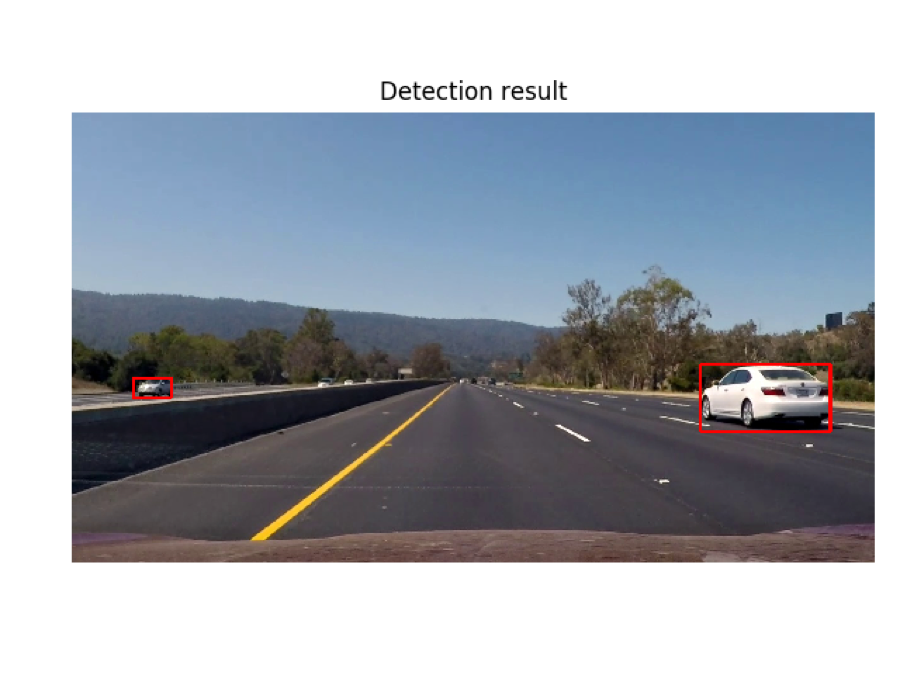
\includegraphics[width=0.9\linewidth]{ssd_consequence}
\end{center}
   \caption{Flow chart of SSD}
\label{fig:2_1_3}
\end{figure}
%-------------------------------------------------------------------------

\subsection{Kalman filter}

Kalman filter is a kind of adaptive filter, which is known as linear quadratic estimation (LQE), is an algorithm that uses a series of measurements observed over time, containing statistical noise and other inaccuracies, and produces estimates of unknown variables that tend to be more accurate than those based on a single measurement alone, by estimating a joint probability distribution over the variables for each timeframe.\\
Kalman filter has following important benefit features~\cite{Kalman}:\\
(1) Predict of object's future location;\\
(2) Correction of the prediction based on new measurements;\\
(3) Reduction of noise introduced by inaccurate detections;\\
(4) Facilitating the process of association of multiple objects to their tracks.

%-------------------------------------------------------------------------
\subsubsection{Algorithm briefly introduction}
The Kalman filters are based on linear dynamical systems discretized in the time domain, and we can make the prediction basing on the following the linear stochastic difference state equation(estimate state equation):
 \begin{equation*}    
    x_t = Ax_{t-1}+w_{t-1}
    \tag{1}
\end{equation*}
with a measurement equation that is:
 \begin{equation*}    
    z_t = Hz_{t-1}+v_{t-1}
    \tag{2}
\end{equation*}
The random variables $w_k$ and $v_k$ represent the process and measurement noise (respectively). They are assumed to be independent (of each other), white, and with normal probability distributions
 \begin{equation*}    
    p(w)\sim N(0,Q)
\end{equation*}
 \begin{equation*}    
    p(v)\sim N(0,R)
\end{equation*}
For the correction and state updating, we introducing the Kalman Gain K, and have the following equations:
 \begin{equation*}    
   K_t=P_tH^T(HP_tH^T+R)^{-1}
   \tag{3}
\end{equation*}
 \begin{equation*}    
   P_t=(1-K_tH)P_{t-1}
   \tag{4}
\end{equation*}
 \begin{equation*}    
   x_t=x_{t-1}+K_{t-1}(z_{t-1}-Hx_{t-1})
   \tag{5}
\end{equation*}
The equations (1)-(5) are the main parts of Kalman Filter. And  
Table.2 shows the meaning of all letters:
\begin{table}
\begin{center}
\begin{tabular}{|c|c|}
\hline
Letter & Meaning \\
\hline\hline
x & Process State \\
\hline
P& estimate error(noise) covariance\\
\hline
A& state transition matrix\\
\hline
Q&  process noise covariance\\
\hline
w& process noise,  w-N(0,Q)\\
\hline
H&  measurement function (matrix)\\
\hline
z& measurement state \\
\hline
R& measurement noise covariance \\
\hline
K& Kalman gain \\
\hline
v& measurement noise, v-N(0,R)\\
\hline
\end{tabular}
\end{center}
\caption{Notation of Kalman filter}
\end{table}

%-------------------------------------------------------------------------
\subsubsection{Car State Prediction}
Using the measurement state we can predict the next state of the tracking car. The information we choose of the car are position p, velocity v and acceleration a, and their relationship are basing one the following equations:
\begin{equation*}    
    p_t=p_{t-1}+v_{t-1}{\delta}_t+\frac{1}{2}a_{t-1}{\delta}_t^2
\end{equation*}
\begin{equation*}    
    v_t = v_{t-1}+a_{t-1}{\delta}_t
\end{equation*}
where the ${\delta}_t$ is the time breaking of each frame.  Write the equations above as matrix form, we have the connection matrix A as following:
\begin{equation*}    
    A = \left[
 \begin{matrix}
   1 & {\delta}_t & \frac{1}{2}{\delta}_t^2 \\
   0 & 1 & {\delta}_t \\
   0 & 0 & 0
  \end{matrix}
  \right] 
\end{equation*}
when write the estimate state as:
\begin{equation*} 
x_t = \left[
    \begin{array}{ccc}
      p_t & v_t & a_t
    \end{array}
\right] 
\end{equation*}
To initialize the value, we choose the velocity and accelerate as 0, and let ${\delta_t}$ equals to 1.
\\Thus, in our project, the dimension of state transition matrix is 12$\times$12 , since there are four locations to be tracked, which is left, down, right and up, representing the four corners of the bounding box, and the matrix dimension of x is 12$\times$1. \\
As for the connection matrix of estimate state and measurement state, we choose :
\begin{equation*} 
H = \left[
    \begin{array}{ccc}
      1 & 0 & 0
    \end{array}
\right] 
\end{equation*}
for we only care about the location of the bounding box. The last step is initializing the noise covariance Q,R randomly, and the value of R shows the confidence of the confidence of prediction.
The results of Kalman Filter prediction are shown as figure \ref{fig:2_1_4}
\begin{figure}[t]
\begin{center}
   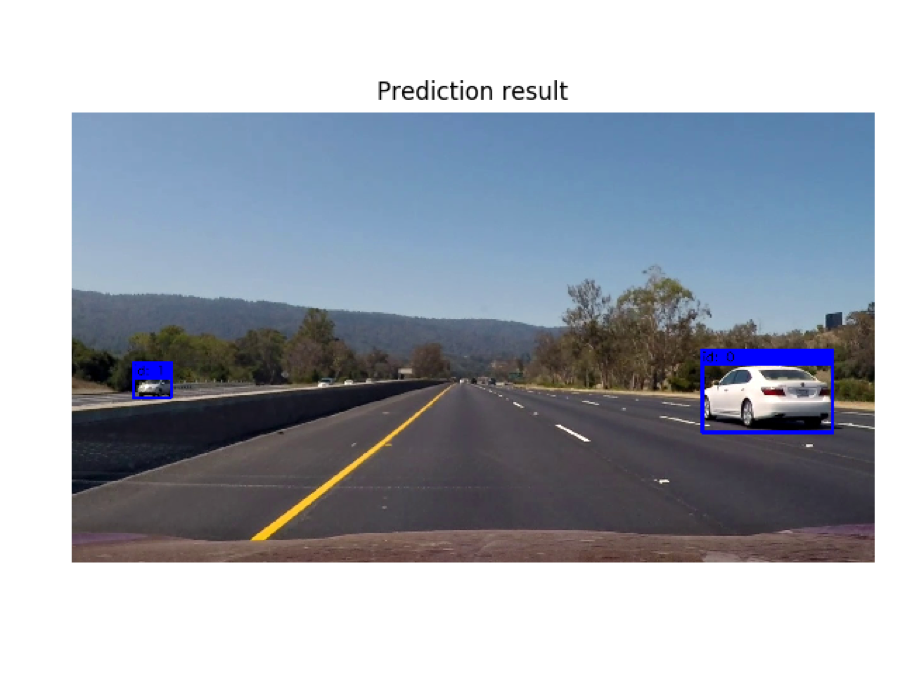
\includegraphics[width=0.9\linewidth]{kalman_r}
\end{center}
   \caption{Result of Kalman filter}
\label{fig:2_1_4}
\end{figure}
%-------------------------------------------------------------------------
\subsection{Conclusion for two algorithms}
Above all are the main idea an process details of car detection and prediction. The main function of our project is to combine the two results with labels to finish the car tracking.

%------------------------------------------------------------------------
\section{Data association and track management}

Previous chapter has introduced how to obtain detection and prediction results given an input image. Notice that for each image, there can be one more cars, so there will be multiple detection and prediction boxes. Thus, a detection-to-tracker assignment is needed to match the results with each other. Then we clarify how to process track management across consecutive frames in the video.

\subsection{Intersection-over-union (IoU)}
Intersection-over-union is an evaluation metric used to measure the accuracy of an object detector given ground truth. We use this parameter to measure the accuracy of detection and prediction results. So in our case, the ground truth is the detection results (boxes) and tracking results (boxes). IoU can be computed as 
\begin{equation*}
\mbox{IoU} = \frac{\mbox{DetectionResults} \cap \mbox{GroundTruth}}{\mbox{DetectionResults} \cup \mbox{GroundTruth}}.
\end{equation*}
For convenience, we call the prediction boxes trackers, and call the detection boxes detections. For each pair of tracker and detection, we can calculate their IoU and thus we can obtain an IoU matrix like shown in figure \ref{fig:3_1_1}.

\begin{figure}[t]
\begin{center}
   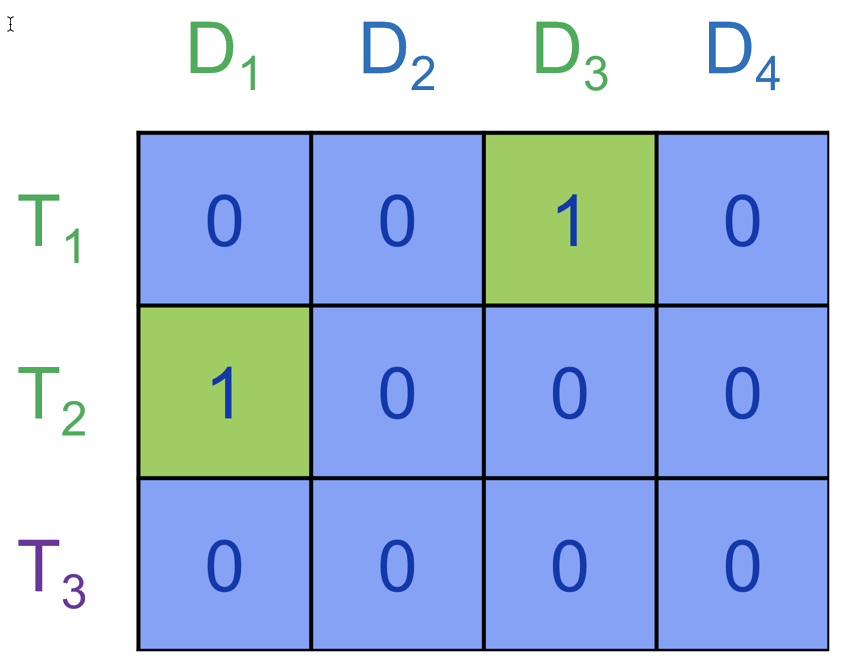
\includegraphics[width=0.4\linewidth]{3_1_1.png}
\end{center}
   \caption{A simple example of IoU matrix with 3 trackers ($T_1$ to $T_3$ and 4 detections ($D_1$ to $D_4$)}
\label{fig:3_1_1}
\end{figure}

\subsection{Detection-to-tracker assignment}
After obtaining the IoU matrix of trackers and detections, we can use Hungarian assignment~\cite{Hungarian1, Hungarian2} to find a maximum weight matching (or minimum weight perfect matching) in the weighted bigraph, which in our case, is the IoU matrix. For our simple example, we can easily figure out that we can maximize the overall IoU weight by matching $D_3$ to $T_1$ and $D_1$ to $T_2$, and $T_3$ and $D_2$, $D_4$ have no matched results. This information will be later used for our tracking management, so we create 3 lists to save the information. List \emph{matched} saves the information of matched results, containing all the matching tuples, which are ($D_3$, $T_1$), ($D_1$, $T_2$). List \emph{unmatched\_detections} saves the information of unmatched detections, which are $D_2$ and $D_4$. List \emph{unmatched\_trackers} saves the information of unmatched trackers, which is $T_3$.

\subsection{Pipeline}
Since our input is a video, we need to capture each frame of the video. This can be done by Python MoviePy package. And then we can obtain the \emph{matched}, \emph{unmatched\_detections} and \emph{unmatched\_trackers} list for each frame using Hungarian assignment. 

\subsubsection{Hits and losses}
The accuracy of SSD is certainly not 100\%, so there will false alarm and missed detection for each frames. False alarm happens when there is a detection box produced by SSD, but in fact there is no car in the bounding box. Missed detection happens when there is a car in the current frame, but there are no matched detection boxes. These two situations can harm the performance of the system. 

In order to solve this, we introduce two important parameters, \emph{min\_hits} and \emph{max\_losses} . We call a tracker has one hit if we have a matched detection and tracker. We call a tracker has one loss if the tracker doesn’t have a matched detection. Using the previous IoU matrix as an example, $T_1$ and $T_2$ has one hit, and $T_3$ has one loss. \emph{Min\_hits} is a constant, standing for the minimum number of consecutive matches to establish a tracker. Similarly, \emph{max\_losses} stands for the maximum number of consecutive losses to delete a current tracker. 

We also introduce another variable to discriminate false alarm and real target. A tracker is called \emph{good tracker} if it has reached \emph{min\_hits}.

\subsubsection{Pipeline diagram}
Pipeline diagram of track management algorithm is shown in figure \ref{fig:3_3_1}.

\begin{figure}[t]
\begin{center}
   \includegraphics[width=1\linewidth]{3_3_1.png}
\end{center}
   \caption{Pipeline diagram of track management algorithm}
\label{fig:3_3_1}
\end{figure}

The inputs are the current frame extracted from the given video, and tracker list, which is the output of the previous frame. Then using SSD we can obtain the detection boxes. Along with the tracking boxes stored in tracker list, we can calculate IoU matrix and using linear assignment to produce \emph{unmatched\_detection} list, \emph{matched} list and \emph{unmatched\_tracker} list. 

\begin{itemize}
\item For each tracker in \emph{unmatched\_detection} list, there is no previous tracking information, so we initialize a new tracker based on detection results and append it to tracker list. Every new tracker will be assigned a new ID sequentially from 0 to 99.
\item For each tracker in \emph{matched} list, we can obtain both detection and prediction results, so we can perform time update and measurement update, and then we have one more hit for the current tracker and set its losses to 0. We also judge if this tracker is a good tracker based on its total number of hits. 
\item For each tracker in \emph{unmatched\_tracker} list, There are no detection results, so we only perform time update, then set its hits to 0, and add 1 to its total number of losses. 
\end{itemize}

In this way we obtain an updated tracker list. And for each tracker in the tracker list, we can judge if the tracker is lost based on the statistics of the hits and losses of the tracker and whether the trackers is a good tracker. For good tracker, the algorithm will track the good tracker for a longer time compared with false alarms (which is bad tracker). If the tracker is lost, we can delete the tracker from the tracker list. Then its ID can be reused for later trackers.


%------------------------------------------------------------------------
\section{Results and Analysis}

Our project achieved several important functionalities, which are tracking one or more cars and assign stable ids separately, removing tracking result in the opposite direction, dealing with car overtaking situation. 

Under the situation that there are cars in the opposite direction, which is unnecessary to track. For automatic driving purpose, cars in the same direction lanes are objects we need to avoid with higher priority.   Some
typical images are shown in figure \ref{fig:4_1} to \ref{fig:4_6}.

\begin{figure}[!h]
\begin{center}
   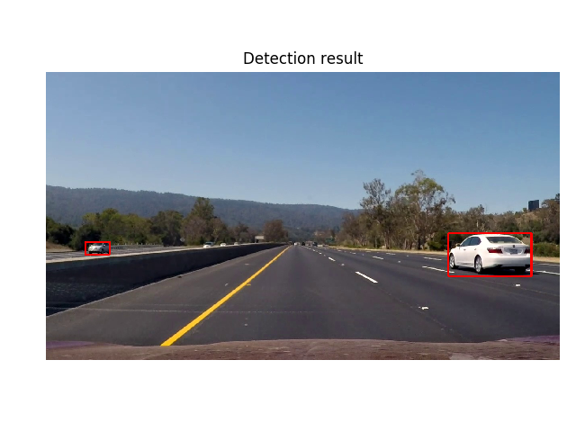
\includegraphics[width=1\linewidth]{__1.png}
\end{center}
   \caption{Detection Result}
\label{fig:4_1}
\end{figure}

\begin{figure}[!h]
\begin{center}
   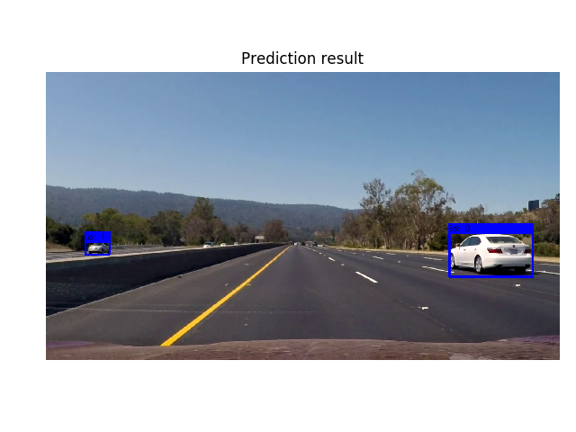
\includegraphics[width=1\linewidth]{__2.png}
\end{center}
   \caption{Prediction Result}
\label{fig:4_2}
\end{figure}

\begin{figure}[h]
\begin{center}
   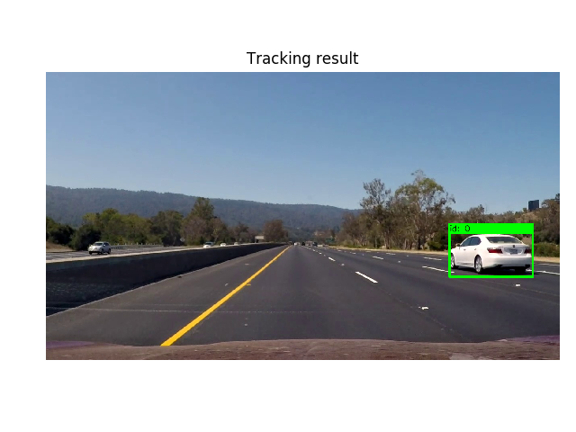
\includegraphics[width=1\linewidth]{__3.png}
\end{center}
   \caption{Tracking Resultt}
\label{fig:4_3}
\end{figure}

\begin{figure}[h]
\begin{center}
   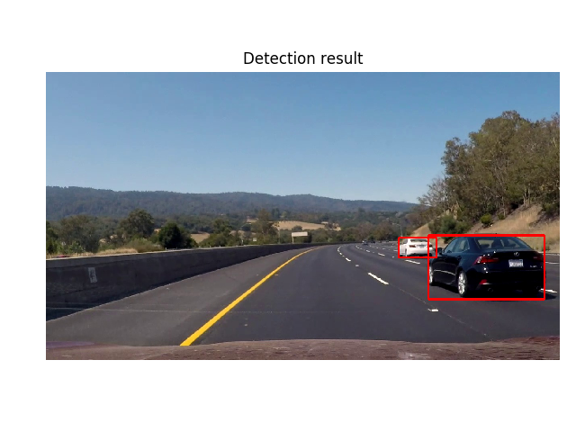
\includegraphics[width=1\linewidth]{__4.png}
\end{center}
   \caption{Multiple Tracking Result}
\label{fig:4_4}
\end{figure}


Our project can make prediction according to the detection result, as shown in \ref{fig:4_1} and \ref{fig:4_2}. In \ref{fig:4_3}, the tracking result of the car in the opposite direction lane disappeared since we set a parameter minhits which needs to be meet to establish a tracker. So the car in the opposite direction which has few appearances can not fulfill the minimum number of consecutive matches to establish a tracker. From the video demo result of detection and tracking, there is a benefit of applying kalman filter which is that even without a consecutive detection, which means the detection is unstable and would disappear in some frames, we can still get a stable and consecutive tracking result. \ref{fig:4_4} shows another main functionality of our project, which are tracking multiple targets and assigning different ids for them. 

\begin{figure}[t]
\begin{center}
   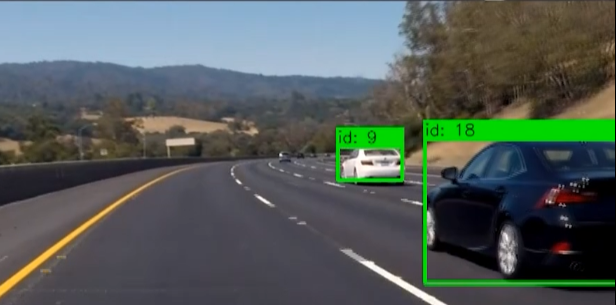
\includegraphics[width=1\linewidth]{overtake1.PNG}
\end{center}
   \caption{Before Overtaking}
\label{fig:4_5}
\end{figure}

\begin{figure}[t]
\begin{center}
   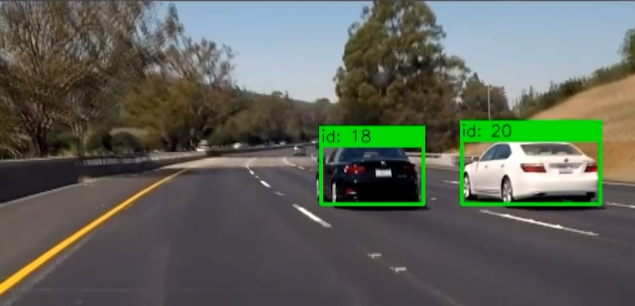
\includegraphics[width=1\linewidth]{overtake2.PNG}
\end{center}
   \caption{After Overtaking}
\label{fig:4_6}
\end{figure}

In the video demo, the black car is going to overtake the white car. From the comparison of \ref{fig:4_5} and \ref{fig:4_6}, it is obvious to conclude that the id of the black car remains unchanged. The white car’s id changed because it has disappeared for a while when the black car blocked it. This tracking results shows that as long as the car keep showing up in our camera view, we can always track it and assign a very stable id for it.

\newpage
{\small
\bibliographystyle{ieee}
\bibliography{egbib}
}

\end{document}
